\documentclass[a4paper,UTF8]{article}
\usepackage{ctex}
\usepackage[margin=1.25in]{geometry}
\usepackage{color}
\usepackage{graphicx}
\usepackage{amssymb}
\usepackage{amsmath}
\usepackage{amsthm}
\usepackage{soul, color, xcolor}
\usepackage{bm}
\usepackage{tcolorbox}
\usepackage{hyperref}
\numberwithin{equation}{section}
%\usepackage[thmmarks, amsmath, thref]{ntheorem}
\theoremstyle{definition}
\newtheorem*{solution}{Solution}
\newtheorem*{prove}{Proof}
\usepackage{multirow}
\usepackage{diagbox}
\usepackage{float}

\def \X {\mathbf{X}}
\def \A {\mathbf{A}}
\def \Q {\mathbf{Q}}
\def \P {\mathbf{P}}
\def \Diag {\textbf{$\Lambda$}}
\def \w {\hat{\boldsymbol{w}}}
\def \y {\boldsymbol{y}}
\def \x {\boldsymbol{x}}
\def \z {\mathbf{z}}
\def \b {\mathbf{b}}
\def \by {\Bar{y}}
\def \H {\mathbf{H}}
\def \I {\mathbf{I}}
\setlength{\parindent}{0pt}
%--

%--
\begin{document}
\title{机器学习导论\ 习题一}
\author{221300079, 王俊童, \href{mailto:221300079@smail.nju.edu.cn}{221300079@smail.nju.edu.cn}}
\maketitle
\section*{作业提交注意事项}
\begin{tcolorbox}
    \begin{enumerate}
        \item[1.] 作业所需的LaTeX及Python环境配置要求请参考: \href{https://www.lamda.nju.edu.cn/ML2024Spring/supplemantary/environment.pdf}{[Link]};
        \item[2.] 请在LaTeX模板中第一页填写个人的学号、姓名、邮箱;
        \item[3.] 本次作业需提交的文件与对应的命名方式为:
            \begin{enumerate}
                \item [(a)] 作答后的LaTeX代码 --- HW1.tex;
                \item [(b)] 由(a)编译得到的PDF文件 --- HW1.pdf;
                \item [(c)] 第三题代码 --- Problem3.py;
                \item [(d)] 第五题代码 --- Problem5.py;
            \end{enumerate}
            请将以上文件{\color{red}\textbf{打包为~学号\_姓名.zip}} (例如 221300001\_张三.zip) 后提交;
        \item[3.] 若多次提交作业, 则在命名~.zip 文件时加上版本号, 例如 221300001\_张三\_v1.zip” (批改时以版本号最高的文件为准);
        \item[4.] 本次作业提交截止时间为 {\color{red}\textbf{ 4 月 2 日23:59:59}}. 未按照要求提交作业, 提交作业格式不正确, {\color{red}\textbf{作业命名不规范}}, 将会被扣除部分作业分数; 除特殊原因 (如因病缓交, 需出示医院假条) 逾期未交作业, 本次作业记 0 分; {\color{red}\textbf{如发现抄袭, 抄袭和被抄袭双方成绩全部取消}};
        \item[5.] 学习过程中, 允许参考 ChatGPT 等生成式语言模型的生成结果, 但必须在可信的信息源处核实信息的真实性; {\color{red}\textbf{不允许直接使用模型的生成结果作为作业的回答内容}}, 否则将视为作业非本人完成并取消成绩;
        \item[6.] 本次作业提交地址为 \href{https://box.nju.edu.cn/u/d/d6a0c7575dc34a7d8e62/}{[Link]}, 请大家预留时间提前上交, 以防在临近截止日期时, 因网络等原因无法按时提交作业.
    \end{enumerate}
\end{tcolorbox}
\newpage

\section{[25pts] Mathematical Foundations}
\begin{enumerate}
    \item[(1)] \textbf{[10pts]} (Derivatives of Matrices) 
    有 $\alpha \in \mathbb{R}$, $\y\in \mathbb{R}^{m\times 1}$, $\x\in \mathbb{R}^{n\times 1}$ 且 $\A\in \mathbb{R}^{n\times n}$. 试完成如下题目\textcolor{blue}{(请给出必要的计算步骤, 否则不予计分)}:  
    \begin{enumerate}
        \item[(a)] \textbf{[5pts]} 若 $\b\in\mathbb{R}^{n\times 1}$ 且 $\alpha=\x^\top\A\x + \b^\top \x$, 试求 $\frac{\partial \alpha}{\partial \x}$.
        \item[(b)] \textbf{[5pts]} 若 $\A$ 可逆, $\A$ 为 $\alpha$ 的函数且 $\frac{\partial \A}{\partial \alpha}$ 已知, 试求 $\frac{\partial \A^{-1}}{\partial \alpha}$.
    \end{enumerate}
    \item[(2)] \textbf{[15pts]} (Statistics) 
    有 $x_1,\cdots,x_n \mathop{\sim}\limits^{iid} \mathcal{N}(\mu, \sigma^2)$. 试完成如下题目: 
    \begin{enumerate}
        \item[(a)] \textbf{[4pts]} 定义 $\bar{x} = \frac{1}{n}\sum\limits_{i=1}^n x_i$. 试证明 $\bar{x}\sim \mathcal{N}(\mu, \frac{\sigma^2}{n})$. 
        \item[(b)] \textbf{[7pts]} 定义 $s^2 = \frac{1}{n-1}\sum\limits_{i=1}^n (x_i - \bar{x})^2$. 试证明 $\frac{(n-1)s^2}{\sigma^2}\sim \chi^2_{n-1}$ 且 $s^2$ 独立于 $\bar{x}$. 
        \item[(c)] \textbf{[4pts]} 试证明 $\frac{\bar{x}-\mu}{s/\sqrt{n}}$ 服从自由度为 $n-1$ 的学生 t 分布. 
    \end{enumerate}
\end{enumerate}

\begin{solution}
    (1.a)$\b\in\mathbb{R}^{n\times 1}$ 且 $\alpha=\x^\top\A\x + \b^\top \x$,此式子并不是二次型,所以需要分开讨论一下:\\
    $\frac{\partial \alpha}{\partial \x} = (a_{11} x_1 + a_{12}x_2 + ... a_{1n}x_n + ... + a_{nn} x_n) + (a_{11} x_1 + a_{21}x_2 + ... a_{n1}x_n + ... + a_{nn} x_n) = (A + A^T)x + b$\\
    (1.b)因为A可逆,由$A A^{-1} = I$,求导之后就可以了,所以有:$\frac{\partial \A^{-1}}{\partial \alpha}=-A^{-1} \frac{\partial\A}{\partial \alpha} A^{-1}$,其中,将我们已知的A对$\alpha$的偏导带入即可\\
    (2.a)由$E(cg(x))=cE(g(x))$可得:$E[\bar{X}] = \frac{1}{n} E[\sum_{i=1}^{n}X_i] = \frac{1}{n} * n E(X) = \frac{n}{n} \mu = \mu$\\
    同理方差可以由公式得到:$Var(cg(x))=c^2 Var(g(x)) = \frac{1}{n^2} Var(\sum_{i=1}^{n}X_i) = \frac{n}{n^2} Var(X) = \frac{1}{n} \sigma^2$\\
    (2.b)首先,卡方分布的定义如下:$X_i$满足从0-1正态分布中的一个样本,$Y=X_1^2+...+X_n^2$是一个服从自由度n的卡方分布.\\
    接下来我们把$s^2$带入式子即可:$\frac{(n-1)s^2}{\sigma^2}=\frac{\sum_{i=1}^{n}(X_i - \bar{x})^2}{\sigma^2}=\frac{\sum_{i=1}^{n}(X_i - \mu - (\bar{x} - \mu))^2}{\sigma^2}$\\
    将上面这个式子的分子展开,按照我们已有的期望进行化简之后可以得到:$=\frac{\sum_{i=1}^{n}(X_i - \mu)^2 - n(\bar{X} - \mu)}{\sigma^2} = \sum_{i=1}^{n}\frac{(X_i - \mu)^2}{\sigma^2} - \frac{(\bar{X} - \mu)^2}{\sigma^2 /n}$\\
    由于上面这$\frac{X_i - \mu}{\sigma} \sim N(0,1),\frac{\bar{X} - \mu}{\sigma / \sqrt{n}} \sim N(0,1)$两个式子都满足0-1正态分布,我们发现进行减法之后正好满足一个n-1的卡方分布.\\
    要证明独立性,只需要证明协方差为0即可:$Cov(s^2,\bar{X})=0$\\
    对于这个题目,就是证明$\bar{X}$与$\bar{X} - X_i$的独立性\\
    $Cov(\bar{X},\bar{X} - X_i) = Cov(\bar{X},\bar{X}) - Cov(\bar{X},X_i) = Var(\frac{1}{n}\sum_{i=1}^{n}X_i)-Cov(\frac{1}{n}\sum_{i=1}^{n}X_i ,X_i) = \frac{\sigma^2}{n} - \frac{\sigma^2}{n} = 0$,由此说明了他们是独立的\\
    (2.c)首先明确t分布的定义:$X \sim N(0,1),Y \sim X^2(n)$ 相互独立,$T = \frac{X}{\sqrt{Y/n}}$满足$T \sim t(n)$\\
    由2.a,2.b可以得到:$\frac{\bar{X} - \mu}{\sigma \sqrt{n}} \sim n(0,1)$且$\frac{(n-1)S^2}{\sigma^2} \sim X^2(n-1)$\\
    可以得到:$\frac{\bar{X} - \mu}{S/\sqrt{n}} = \frac{\bar{X} - \mu}{\sigma / \sqrt{n}}/ \sqrt{\frac{(n-1)S^2}{\sigma^2 (n-1)}} \sim t(n-1)$\\
\end{solution}


\newpage
\section{[10pts] Performance Measure}
性能度量是衡量模型泛化能力的评价标准, 在对比不同模型的能力时, 使用不同的性能度量往往会导致不同的评判结果.
请仔细阅读《机器学习》第二章 2.3.2 节. 在书中, 我们学习并计算了模型的二分类性能度量. 下面我们给出一个多分类 (三分类) 的例子, 请根据学习器的具体表现, 回答如下问题.
\begin{table}[ht]
    \centering
    \caption{类别的真实标记与预测标记}
    \label{tab:samples1}
    \begin{tabular}{|l|l|l|l|l|}
    \hline
    \diagbox{真实类别}{预测类别}   & 第一类 & 第二类 & 第三类 \\ \hline
    第一类 & 9   & 0   & 2   \\ \hline
    第二类 & 2   & 8   & 1   \\ \hline
    第三类 & 0   & 0   & 7   \\ \hline
    \end{tabular}
\end{table}
\begin{enumerate}
    \item[(1)] \textbf{[3pts]}  如表~\ref{tab:samples1} 所示, 请计算该学习器的错误率及精度.
    \item[(2)] \textbf{[3pts]}  请分别计算宏查准率, 宏查全率, 微查准率, 微查全率.
    \item[(3)] \textbf{[4pts]}  分别用宏查准率, 宏查全率, 微查准率, 微查全率计算宏$F1$度量, 微$F1$度量.
\end{enumerate}

\begin{solution}
    首先可以得到以下的一些信息:\\
    第一类样本个数11,第二类样本个数11,第三类样本个数7,总样本数29.\\
    (2.1)正确样本数:9+8+7 = 24个,错误数量5个,所以可得:$error = 5/29 \approx 0.1724$,$precise = 1 - error = 0.8276$\\
    (2.2)对第1类:$TP_1 =9,FN_1 = 2,FP_1 = 2,TN_1 = 16$\\
    对第2类:$TP_2 =8,FN_2 = 3,FP_2 = 0,TN_2 = 18$\\
    对第3类:$TP_3 =7,FN_3 = 0,FP_3 = 3,TN_3 = 19$\\
    micro-P = $\frac{\bar{TP}}{\bar{TP} + \bar{FP}}=$(9+8+7)/(9+8+7)+(2+0+3) = 24/24+5 $\approx$ 0.8276\\
    micro-R = $\frac{\bar{TP}}{\bar{TP} + \bar{FN}}=$(9+8+7)/(9+8+7)+(2+3+0) = 24/24+5 $\approx$ 0.8276\\
    然后分别计算:$P = \frac{TP}{TP + FP},R = \frac{TP}{TP + FN}$\\
    第一类:$P_1 = 9/11 = 0.8182, R_1 = 9 / 11 = 0.8182 $\\
    第二类:$P_2 = 8/8  = 1, R_2 = 8 / 11 = 0.7273 $\\
    第三类:$P_3 = 7/10 = 0.7, R_3 = 7 / 7 = 1 $\\
    macro-P = $\sum_{i=1}^{3}P_i$ = (0.8182 + 1 + 0.7)/3 = 0.8394\\
    macro-R = $\sum_{i=1}^{3}R_i$ = (0.8182 + 0.7273 + 1)/3 = 0.8485\\
    (2.3)根据公式可得:\\
    micro-F1 = 2*0.8276*0.8276 / (0.8276+0.8276) = 1.3698 / 1.6552 = 0.8275\\
    macro-F1 = 2*0.8394*0.8495 / (0.8394+0.8495) = 1.4261 / 1.6889 = 0.8443\\
\end{solution}


\newpage
\section{[20pts] Cross Validation \& Model Selection}
机器学习常涉及两类参数: 一类是算法的参数, 亦称``超参数'', 如对数几率回归模型训练的迭代总次数; 另一类是模型的参数, 如对数几率回归模型的 $\mathbf{w}$ 与 $b$. 大多数学习算法的性能都会受到超参数设置的影响. 在《机器学习》第二章 2.2.2 节中介绍了一种模型评估方法 --- 交叉验证, 它也经常被用于算法的参数调节. 下面, 我们尝试通过交叉验证, 寻找在所给数据集上最适合岭回归分类器 (RidgeClassifier) 的超参数 $\alpha$. 请仔细阅读代码框架 Problem3.py, 补全空缺的代码片段, 实现以下的功能并回答相关问题.
\begin{enumerate}
    \item [(1)] \textbf{[6pts]} 补全空缺代码, 实现 k 折交叉验证方法.
    \item [(2)] \textbf{[4pts]} 通过单次 10 折交叉验证, 评估不同 $\alpha$ 值对分类器的性能影响. 请将生成的 cross\_validation.png 图表放置在解答区域.
    \item [(3)] \textbf{[5pts]} 基于上一题的结果选取最优的 $\alpha$ 值, 并计算模型在测试集上的分类精度. 请汇报选取的最优超参数 $\alpha$ 的取值与对应的分类精度.
    \item [(4)] \textbf{[5pts]} 基于上述实验, 阅读《机器学习》2.2.4 节的内容, 简要谈谈在评估学习算法的泛化性能时, 数据集划分与超参数调节的大致流程.
\end{enumerate}

\begin{solution}
    %%%%% use following code to insert the picture %%%%%
    (3.1)我已完成任务\\
    (3.2)图如下\\
    \begin{figure}[H]
        \centering
        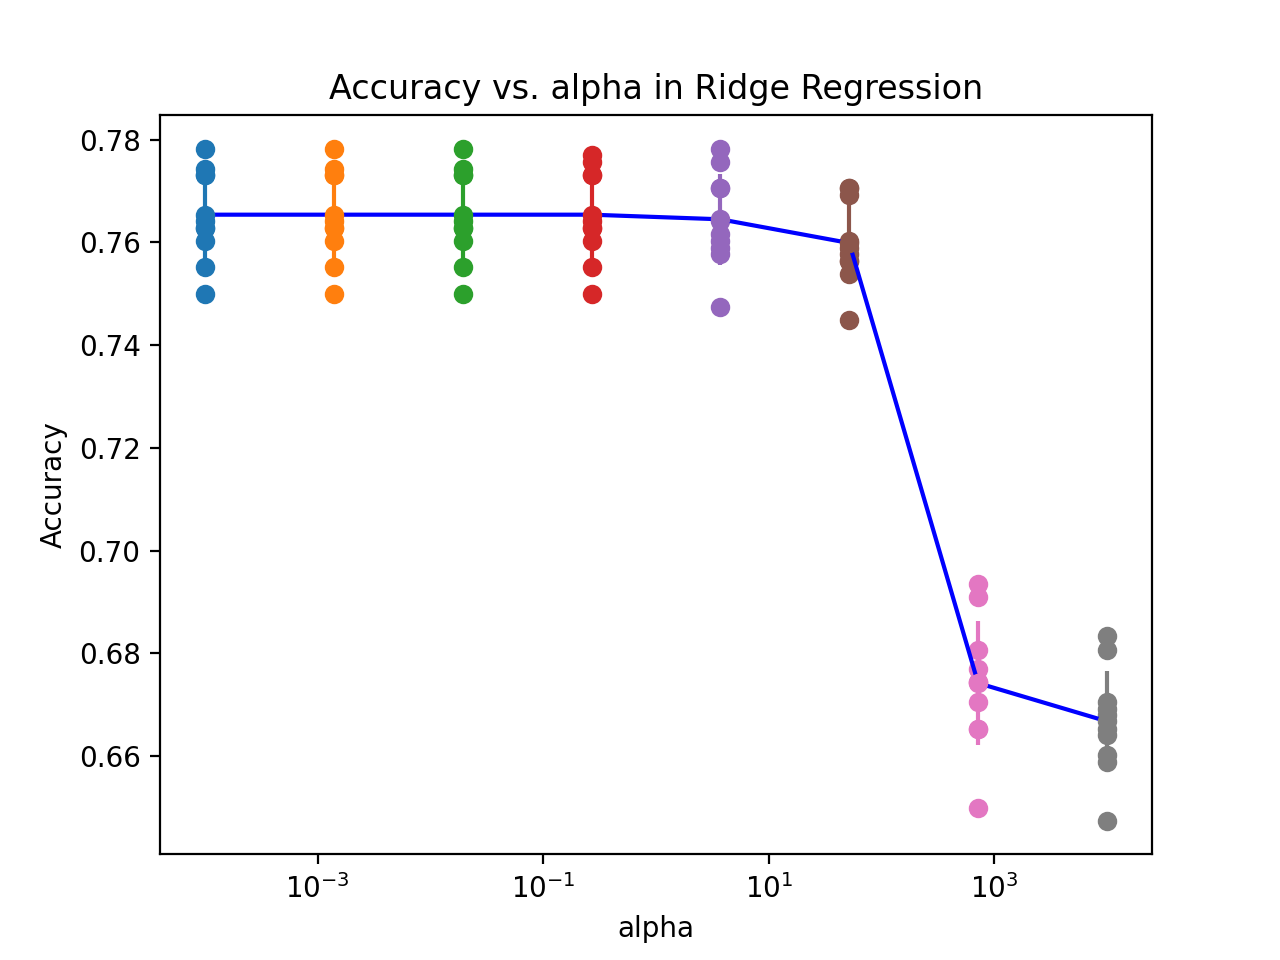
\includegraphics[width=0.8\textwidth]{cross_validation.png}\\
        \caption{Cross Validation}
        \label{fig:cv}
    \end{figure}
    (3.3)我已完成任务.Best alpha = 0.0001(感觉都差不多?0.0001和0.001), accuracy on test set = 0.7827\\
    (3.4)数据集划分主要是要把数据集划分为训练集和测试集,训练集用来训练模型,测试集用来评估模型的准确性。当然也有在训练集上面进行评估的比如这个题就是如此要求。
    在一般的划分中,我们一般划分为4个部分,$X_train,X_test,y_train,y_test$,在其中,test是所有测试集的属性加上label,train是训练集上的属性加上label。X是不包括label的,y是label,
    这样的话数据集就被划分为了4个部分供我们使用。\\
    关于超参数的选择上,根据书中说的,其实我们选择的超参数并不能保证一定最优,因为超参数在基于实数域的基础上选择的,并不一定是我们所要求的一定的最优解。我们只能从一些候选的超参数里面来进行“折中”,这样才能获得
    最好的学习性能。若超参数的个数过多,则根据要选的超参数集合来看,复杂度会指数递增,这显然是很麻烦的。所以基于超参数的选择上,还需妥善的考虑和衡量。
\end{solution}


\newpage
\section{[25pts] ROC \& AUC}
ROC 曲线与其对应的 AUC 值可以反应分类器在一般情况下泛化性能的好坏. 请仔细阅读《机器学习》第二章 2.3.3 节,并完成本题(\textcolor{blue}{请按定义给出必要的计算步骤, 否则不予计分}; 本题涉及的 ROC 曲线手绘或编程绘制均可).
\begin{table}[ht]
    \centering
    \caption{样例的真实标记与预测}
    \begin{tabular}{c|ccccccccc}
        \hline 样例 & $x_1$ & $x_2$ & $x_3$ & $x_4$ & $x_5$ & $x_6$ & $x_7$ \\
        \hline 标记 & 0 & 1 & 0 & 1 & 0 & 1 & 0 \\
        \hline 分类器输出值 & 0.32 & 0.89 & 0.63 & 0.32 & 0.25 & 0.66 & 0.48 \\
        \hline
    \end{tabular}
    \label{tab:samples}
\end{table} 
\begin{enumerate}
    \item[(1)] \textbf{[5pts]}  如表~\ref{tab:samples} 所示, 第二行为样例的真实标记, 第三行为某分类器对样例的预测结果. 请根据上述结果, 绘制分类器在该样例集合上的 ROC 曲线, 并计算其对应的 AUC 值.
    \item[(2)] \textbf{[6pts]}  除表~\ref{tab:samples} 外另有负类样本 $x_8$, 预测值为 0.8. 请绘制此时的 ROC 曲线, 并计算其对应的 AUC 值. 试分析增加一个预测值高的负类样本对 AUC 带来的影响及原因. 
    \item[(3)] \textbf{[6pts]}  除表~\ref{tab:samples} 外另有正类样本 $x_8$, 预测值为 0.8. 请绘制此时的 ROC 曲线, 并计算其对应的 AUC 值. 试分析增加一个预测值高的正类样本对 AUC 带来的影响及原因, 并相比上问, 分析这两种情况下 AUC 值的变化幅度差异. 
    \item[(4)] \textbf{[8pts]}  试证明对有限样例成立\textcolor{blue}{(请给出详尽的证明过程, 直接使用书中结论不计分)}:
    \begin{equation}
        \label{eq:auc}
            \text{AUC} = \frac{1}{m^+m^-}\sum_{x^+\in D^+}\sum_{x^-\in D^-}\left(\mathbb{I}\left\{f(x^+) > f(x^-)\right\}+\frac{1}{2}\mathbb{I}\left\{f(x^+)=f(x^-)\right\}\right).
    \end{equation}    
\end{enumerate}

\begin{solution}
    (4.1)图像如下所示\\
    \begin{figure}[H]
        \centering
        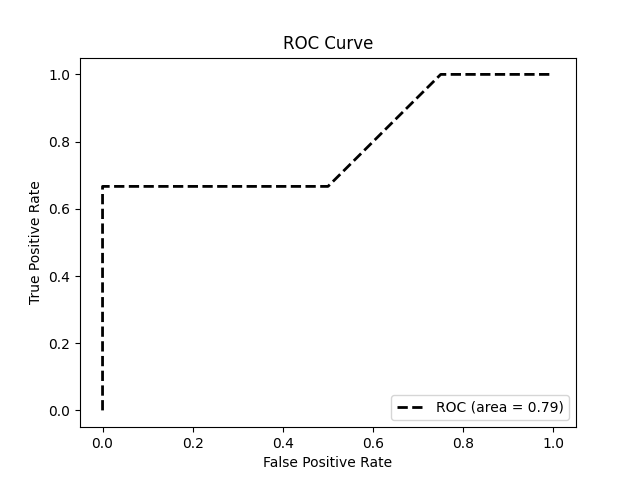
\includegraphics[width=0.7\textwidth]{roc_drawing.png}\\
        \caption{ROC Curve}
        \label{fig:roc_drawing}
    \end{figure}
    AUC: 0.79\\
    (4.2)图像如下所示\\
    \begin{figure}[H]
        \centering
        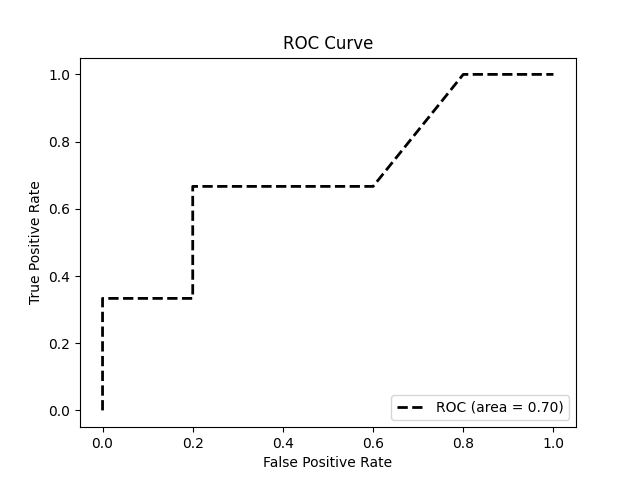
\includegraphics[width=0.7\textwidth]{roc_drawing1.png}\\
        \caption{ROC Curve}
        \label{fig:roc_drawing_0.8}
    \end{figure}
    AUC: 0.70\\
    显然加入一个负类样本,并没有被验证正确,一个负类样本被预测为了一个正类,根据FPR的公式,这是会影响FP的,而FP增加了,显然在一个从高到低排序的分析过程中,这个值第二个会被选到,然后发现错了,产生一个平移,所以这里出现了拐点。这就可以解释这个为啥变小了\\
    (4.3)图像如下所示\\
    \begin{figure}[H]
        \centering
        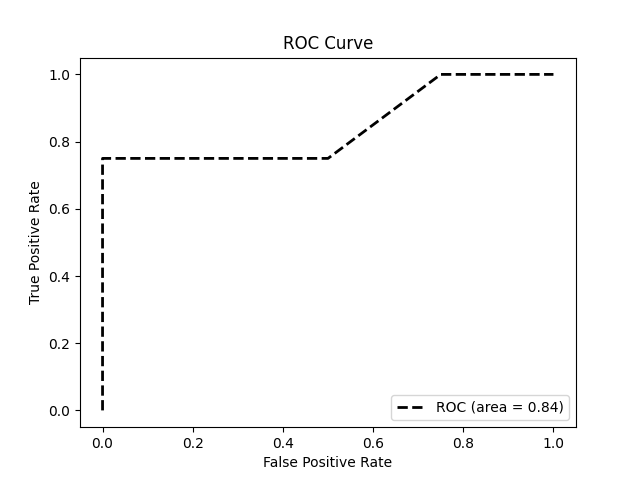
\includegraphics[width=0.7\textwidth]{roc_drawing2.png}\\
        \caption{ROC Curve}
        \label{fig:roc_drawing_0.8}
    \end{figure}
    AUC: 0.84\\
    显然,AUC变高了,说明对于新加入的一个0.8的类,这是被预测为正类的,所以根据公式纵轴$TPR = \frac{TP}{TP+FN}$这个公式实际是变高了,
    所以纵轴是有变高的,所以我们获得的FPR并没有变,所以AUC变大了\\
    (4.4)关于AUC的推导,我们考虑一个梯形面积计算公式,根据书上所说:AUC = 1 - $l_{rank}$,我们只需要推出$l_{rank}$的公式就可以了:\\
    $l_{rank} = \frac{1}{m^+m^-}\sum_{x^+\in D^+}\sum_{x^-\in D^-}\left(\mathbb{I}\left\{f(x^+) < f(x^-)\right\}+\frac{1}{2}\mathbb{I}\left\{f(x^+)=f(x^-)\right\}\right)$\\
    $= \frac{1}{m^+m^-}\sum_{x^+\in D^+}\left(  \sum_{x^-\in D^-} \mathbb{I}\left\{f(x^+) < f(x^-)\right\}+ \sum_{x^-\in D^-}\frac{1}{2}\mathbb{I}\left\{f(x^+)=f(x^-)\right\}\right)$\\
    $= \sum_{x^+\in D^+}\frac{1}{2}\frac{1}{m^+}\left( \frac{2}{m^-} \sum_{x^-\in D^-} \mathbb{I}\left\{f(x^+) < f(x^-)\right\}+ \frac{1}{m^-}\sum_{x^-\in D^-}\mathbb{I}\left\{f(x^+)=f(x^-)\right\}\right)$\\
    对于这个式子,除去第一个求和符号,后面就应该是与y轴围成的梯形面积。其中,根据ROC图我们可以知道$\frac{1}{m^+}$这个东西就是所谓的高,然后我们需要下底和上底\\
    对于上底来说,我们每次增加一个FP就会有一个长度,而这个长度是跟我们的$\frac{1}{m^-}$有关的,所以我们可以得到上底的推导公式:\\
    $upper-line = \frac{1}{m^-} \sum_{x^-\in D^-} \mathbb{I}\left\{f(x^+) < f(x^-)\right\}$\\
    同理,下底的公式就是大于等于假正例的个数:\\
    $under-line = \frac{1}{m^-} \sum_{x^-\in D^-} \mathbb{I}\left\{f(x^+) < f(x^-)\right\} + \sum_{x^-\in D^-} \mathbb{I}\left\{f(x^+) = f(x^-)\right\}$\\
    这样我们就证明了这个$l_{rank}$就是我们需要的面积,用1减去它就是AUC了\\
\end{solution}


\newpage
\section{[20pts] Logistic Regression}
对数几率回归 (Logistic Regression) 是常用的分类学习算法, 通常使用 AUC 值评估其分类性能. 下面, 我们利用 Python 实现二分类的对数几率回归模型, 并采用牛顿法进行模型的优化求解. 请仔细阅读代码框架 Problem5.py, 补全空缺的代码片段, 实现以下的功能并回答相关问题.
\begin{enumerate}
    \item[(1)] \textbf{[5pts]} 实现 $\ell(\mathbf{\beta})$ 关于 $\mathbf{\beta}$ 的二阶导数的计算. (即书中公式 3.31)\\提示: 可以参考框架代码中 $\ell(\mathbf{\beta})$ 关于 $\mathbf{\beta}$ 的一阶导数的计算方法.
    \item[(2)] \textbf{[5pts]} 实现牛顿法的迭代步骤. (即书中公式 3.29)
    \item[(3)] \textbf{[5pts]} 实现基于参数 $\mathbf{\beta}$, 计算 $\mathbf{X}$ 对应的类别概率的方法.
    \item[(4)] \textbf{[5pts]} 绘制训练后的模型在测试集上的 ROC 曲线图, 并汇报对应的 AUC 数值 (保留四位小数). 请将生成的 roc.png 图片放置在解答区域.\\提示: 若你未能完成 (1-3) 题, 你可以使用 sklearn 的对数几率回归模型作为替代.
\end{enumerate}

\begin{solution}
    (5.1,2,3)我已经在代码里面实现了前3问的所有内容\\
    (5.4)我实现了画图:我用了2个方式都画了图来检验我的方法的正确性:
    \begin{figure}[H]
        \centering
        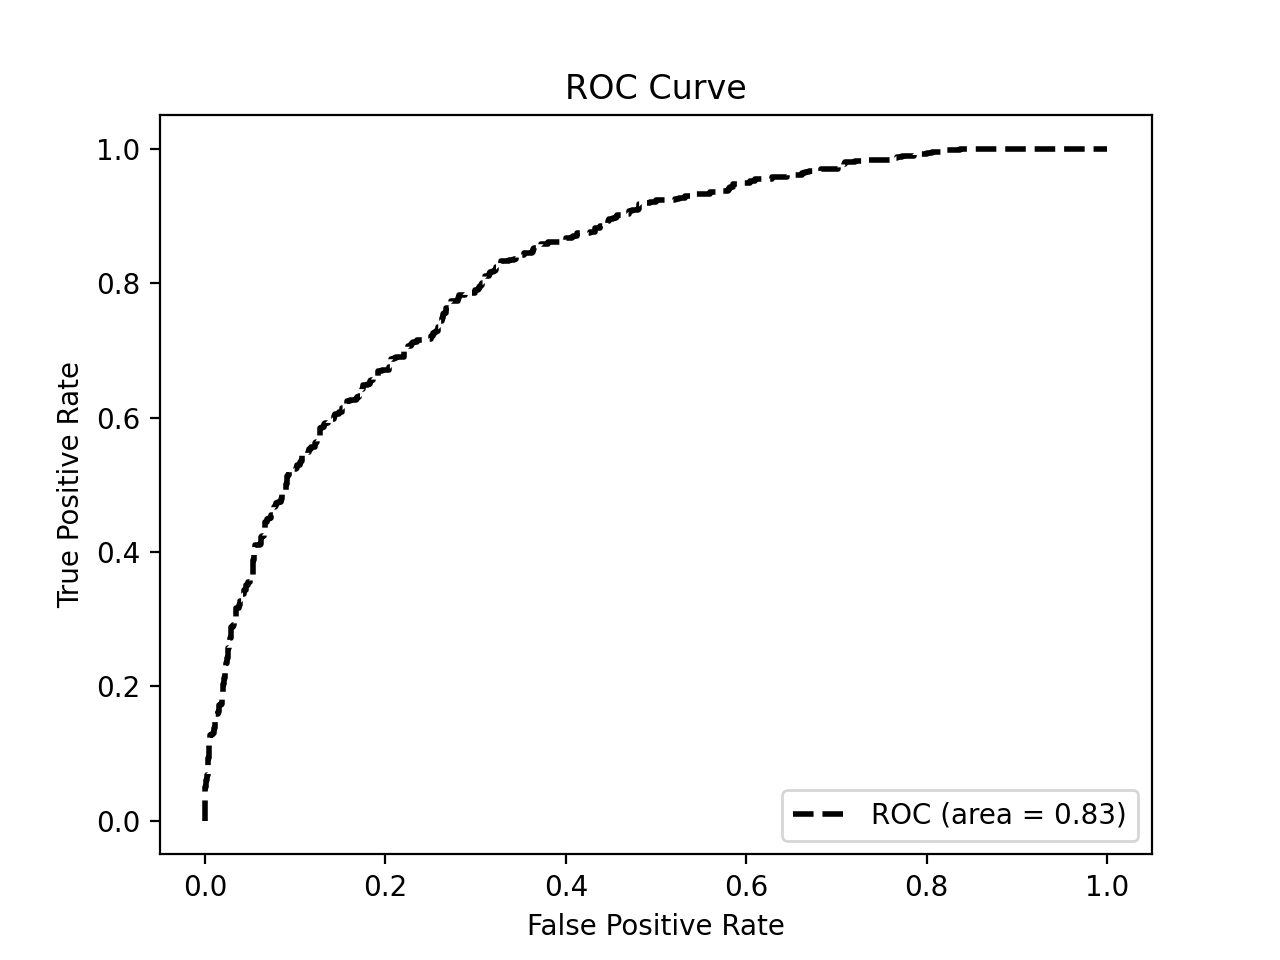
\includegraphics[width=0.7\textwidth]{roc_mylog.png}
        \caption{ROC Curve from mylog}
        \label{fig:roc}
    \end{figure}
    \begin{figure}[H]
        \centering
        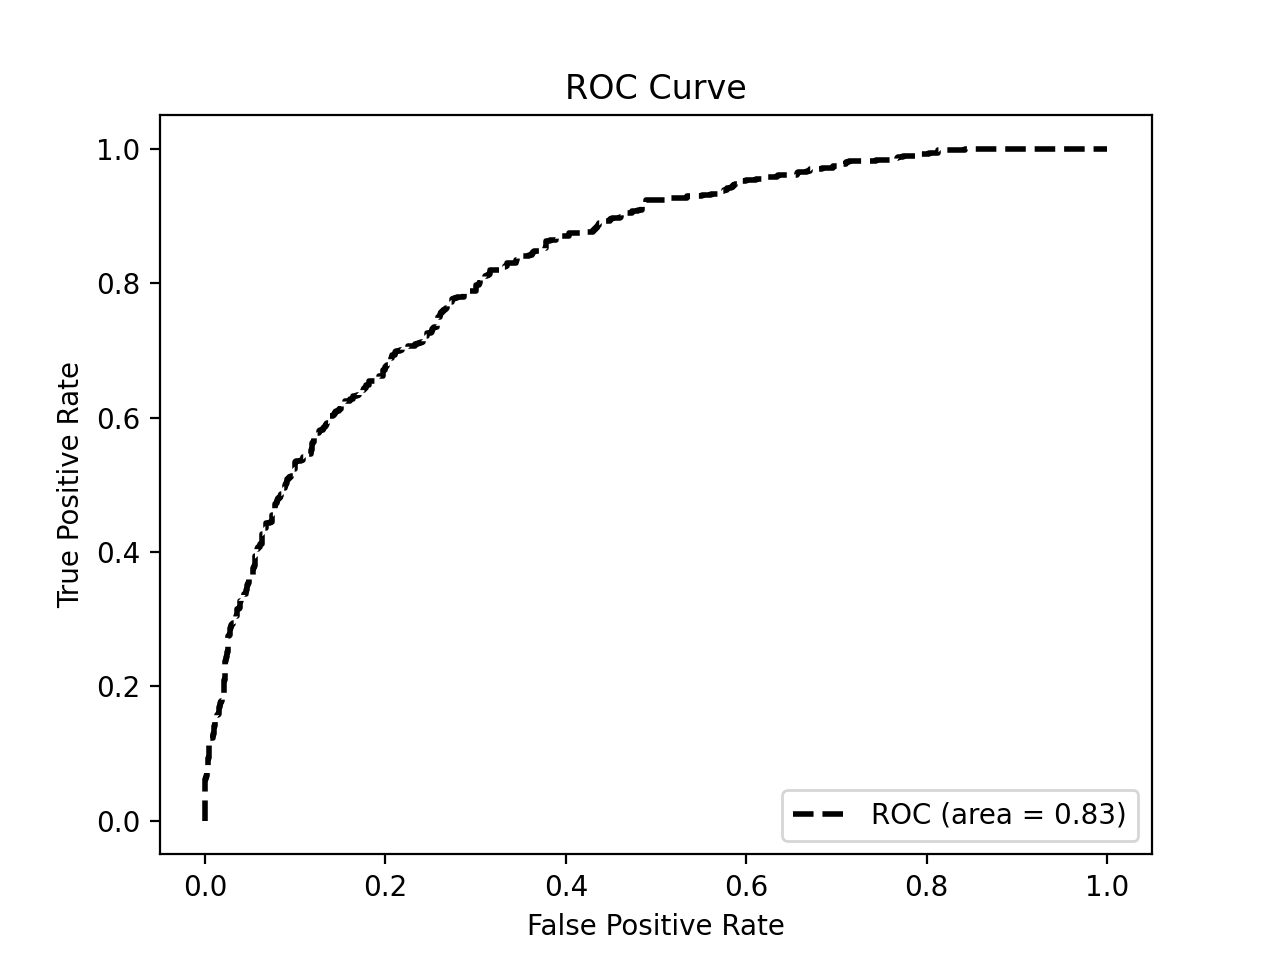
\includegraphics[width=0.7\textwidth]{roc_sklearn.png}
        \caption{ROC Curve from sklearn}
        \label{fig:roc1}
    \end{figure}
\end{solution}


\newpage
\section*{Acknowledgments}
允许与其他同样未完成作业的同学讨论作业的内容, 但需在此注明并加以致谢; 如在作业过程中, 参考了互联网上的资料或大语言模型的生成结果, 且对完成作业有帮助的, 亦需注明并致谢.
\end{document}